\documentclass[a4paper]{report}
\author{Jure Kos}
\title{Vaja 43, Vsiljeno nihanje nihajnega kroga}
\date{22.4.2022}
\usepackage{graphicx}
\graphicspath{ {./images/} }

\begin{document}

\maketitle

\chapter*{Uvod}
Električno nihanje v nihajnem krogu zelo spominja na nihanje na vijačno vzmet, kjer bi napetost predstavljala odmik odmik vzmeti in tok hitrosti uteži. Električna energija kondenzatorja ustreza prožnostni energiji vzmeti in magnetna energija kinetični energiji uteži.\\

Nihanje nihajnega kroga (podobno kakor pri mehaničnem nihalu) po določenem času izzveni, če ga samo enkrat vzbudimo. V kolikor v njem stalno vzbujamo sinusno nihanje, lahko opazujemo vsiljeno nihanje.  Da bi vsiljeno nihanje lahko opazovali, nihajni krog induktivno sklopimo z oscilatorjem in spreminjamo ali frekvenco vsiljene sinusne napetosti ali pa lastno frekvenco nihajnega kroga. Z osciloskopom lahko izmerimo amplitudo inducirane napetosti ter fazno razliko med napetostjo na kondenzatorju nihajnega kroga in napetostjo oscilatorja.

\chapter*{Naloga}
1. Z osciloskopom opazovati vzbujeno nihanje v nihajnem krogu, ki je induktivno vezan z oscilatorjem. Določiti resonančno krivuljo pri različnih stopnjah dušenja. \\
\noindent 2. Opazovati z osciloskopom Lissajoujeve figure in oceniti fazne razlike med inducirano napetostjo in vzbujeno napetostjo.

\section*{Potrebščine}
1. Osciloskop,\\
2. Oscilator s frekvenco $\nu$ = 600 kHz,\\
3. Resonančni krog, \\
4. Umeritvena krivulja za vrtljivi kondenzator, \\
5. Upori 5 $\Omega$, 10 $\Omega$ in 20 $\Omega$.


\chapter*{Meritve}

Za $R = 0 \Omega$
\begin{center}
	\begin{tabular}{ |c|c| } 
 \hline
 C [pF] & U[mV] \\
 \hline
 	445   & 240 \\
    510   & 400 \\
    534   & 680 \\
    550   & 1050 \\
    560   & 1180 \\
    565   & 1630 \\
    580   & 2350 \\
    585   & 4050 \\
    592   & 4650 \\
    599   & 2750 \\
    606   & 1800 \\
    613   & 1250 \\
    650   & 600 \\
    710   & 250 \\
 \hline
	\end{tabular}
\end{center}



za $R = 5 \Omega$
\begin{center}
	\begin{tabular}{ |c|c| } 
 \hline
 C [pF] & U[mV] \\
 \hline
 	320   & 140 \\
    445   & 220 \\
    510   & 390 \\
    534   & 600 \\
    542   & 660 \\
    550   & 820 \\
    560   & 960 \\
    565   & 1200 \\
    580   & 1480 \\
    585   & 1750 \\
    592   & 1850 \\
    599   & 1750 \\
    606   & 1550 \\
    613   & 1200 \\
    620   & 930 \\
    606   & 770 \\
    627   & 650 \\
    650   & 500 \\
    710   & 270 \\
 \hline
	\end{tabular}
	\end{center}



za $R = 10 \Omega$
\begin{center}
	\begin{tabular}{ |c|c| } 
 \hline
 C [pF] & U[mV] \\
 \hline
 	445   & 220 \\
    510   & 370 \\
    534   & 550 \\
    550   & 700 \\
    565   & 8550 \\
    580   & 980 \\
    585   & 1060 \\
    592   & 1100 \\
    606   & 960 \\
    613   & 880 \\
    606   & 660 \\
    650   & 480 \\
    710   & 250 \\
 \hline
	\end{tabular}
\end{center}



za $R = 20\Omega$
\begin{center}
	\begin{tabular}{ |c|c| } 
 \hline
 C [pF] & U[mV] \\
 \hline
 	445   & 210 \\
    510   & 320 \\
    534   & 460 \\
    542   & 500 \\
    550   & 540 \\
    560   & 570 \\
    565   & 600 \\
    580   & 610 \\
    585   & 640 \\
    592   & 640 \\
    599   & 620 \\
    606   & 610 \\
    613   & 570 \\
    634   & 460 \\
    650   & 410 \\
    685   & 300 \\
    710   & 250 \\
 \hline
	\end{tabular}
\end{center}


\chapter*{Računi}

\[\nu_0 = \frac{1}{\sqrt{LC}}\Rightarrow L_0=\frac{1}{\nu_o C_0^2}=4,8\cdot10^{-12}H\]

\begin{figure}[htp]
    \centering
    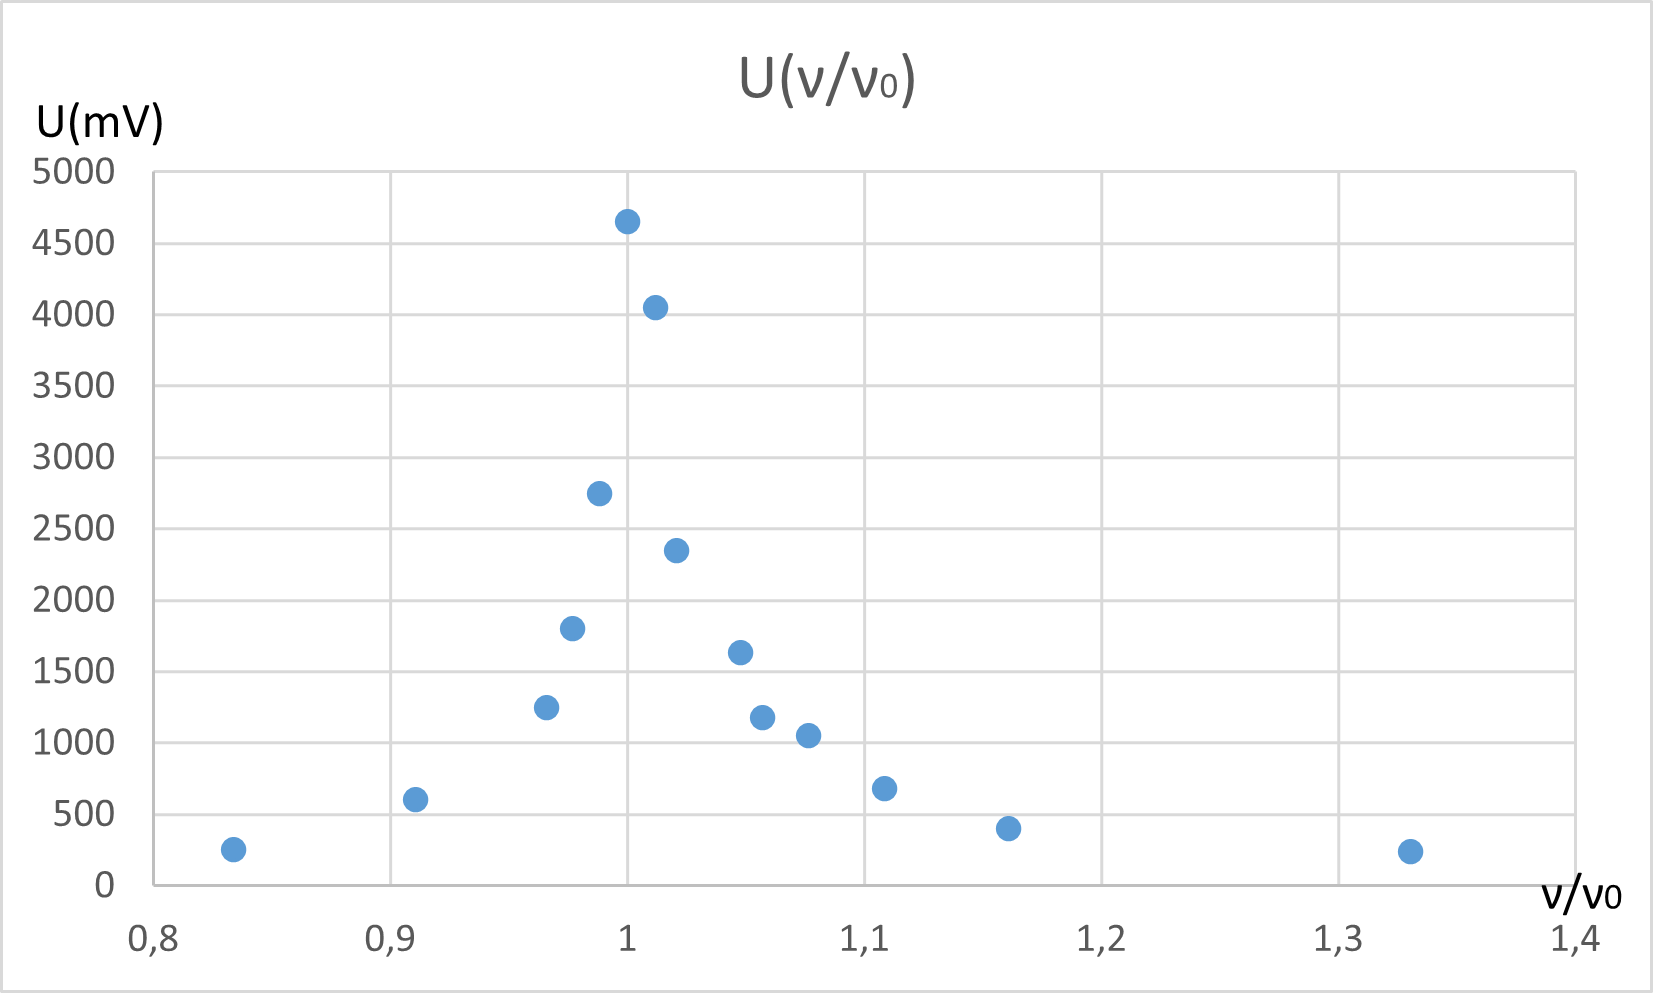
\includegraphics[width=\textwidth]{R = 0.png}
    \caption{R = 0 $\Omega$}
    \label{fig:galaxy}
\end{figure}

\begin{figure}[htp]
    \centering
    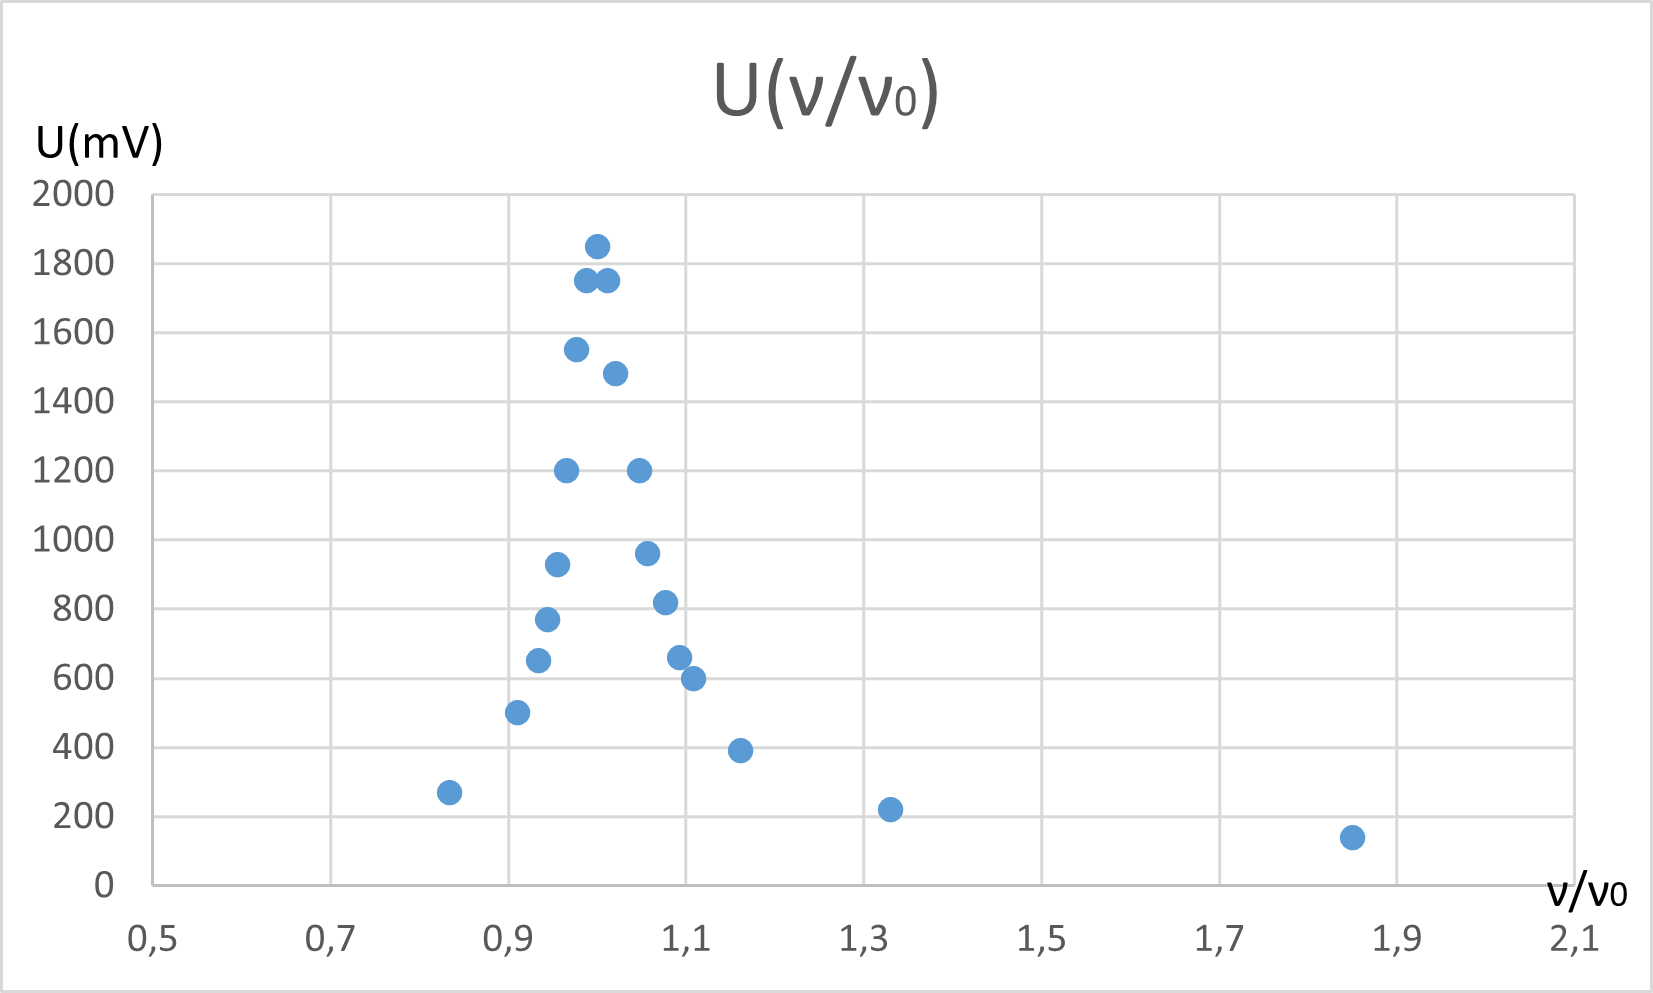
\includegraphics[width=\textwidth]{R = 5.png}
    \caption{R = 5 $\Omega$}
    \label{fig:galaxy}
\end{figure}

\begin{figure}[htp]
    \centering
    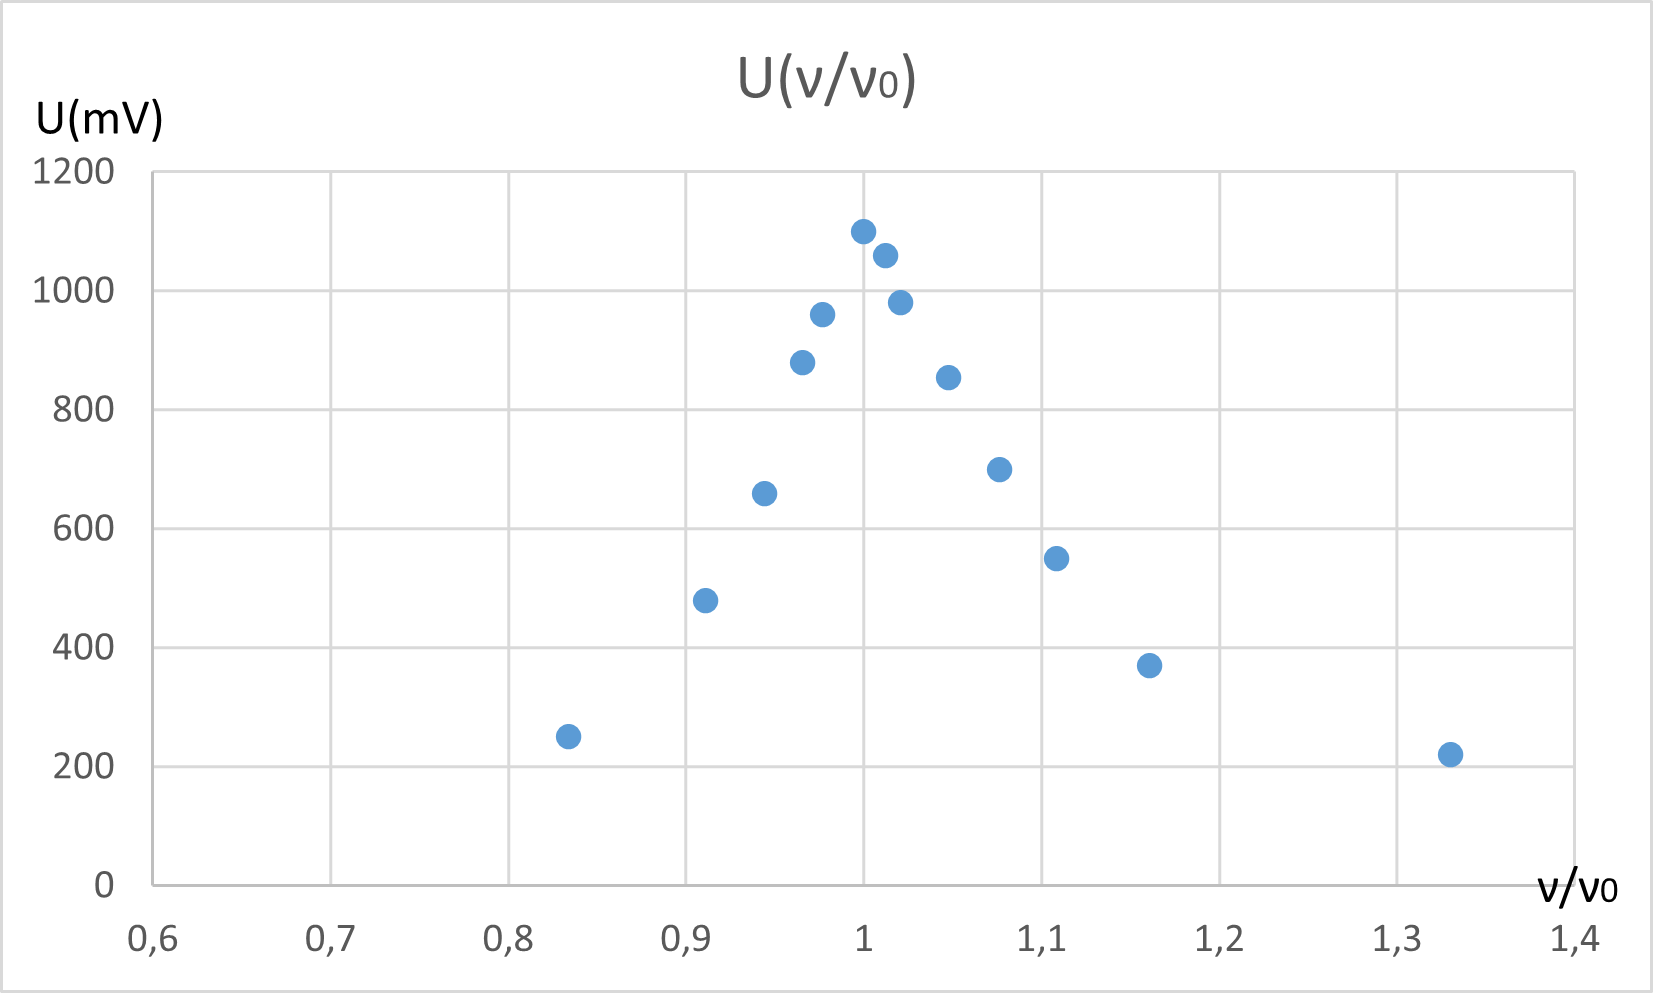
\includegraphics[width=\textwidth]{R = 10.png}
    \caption{R = 10 $\Omega$}
    \label{fig:galaxy}
\end{figure}

\begin{figure}[htp]
    \centering
    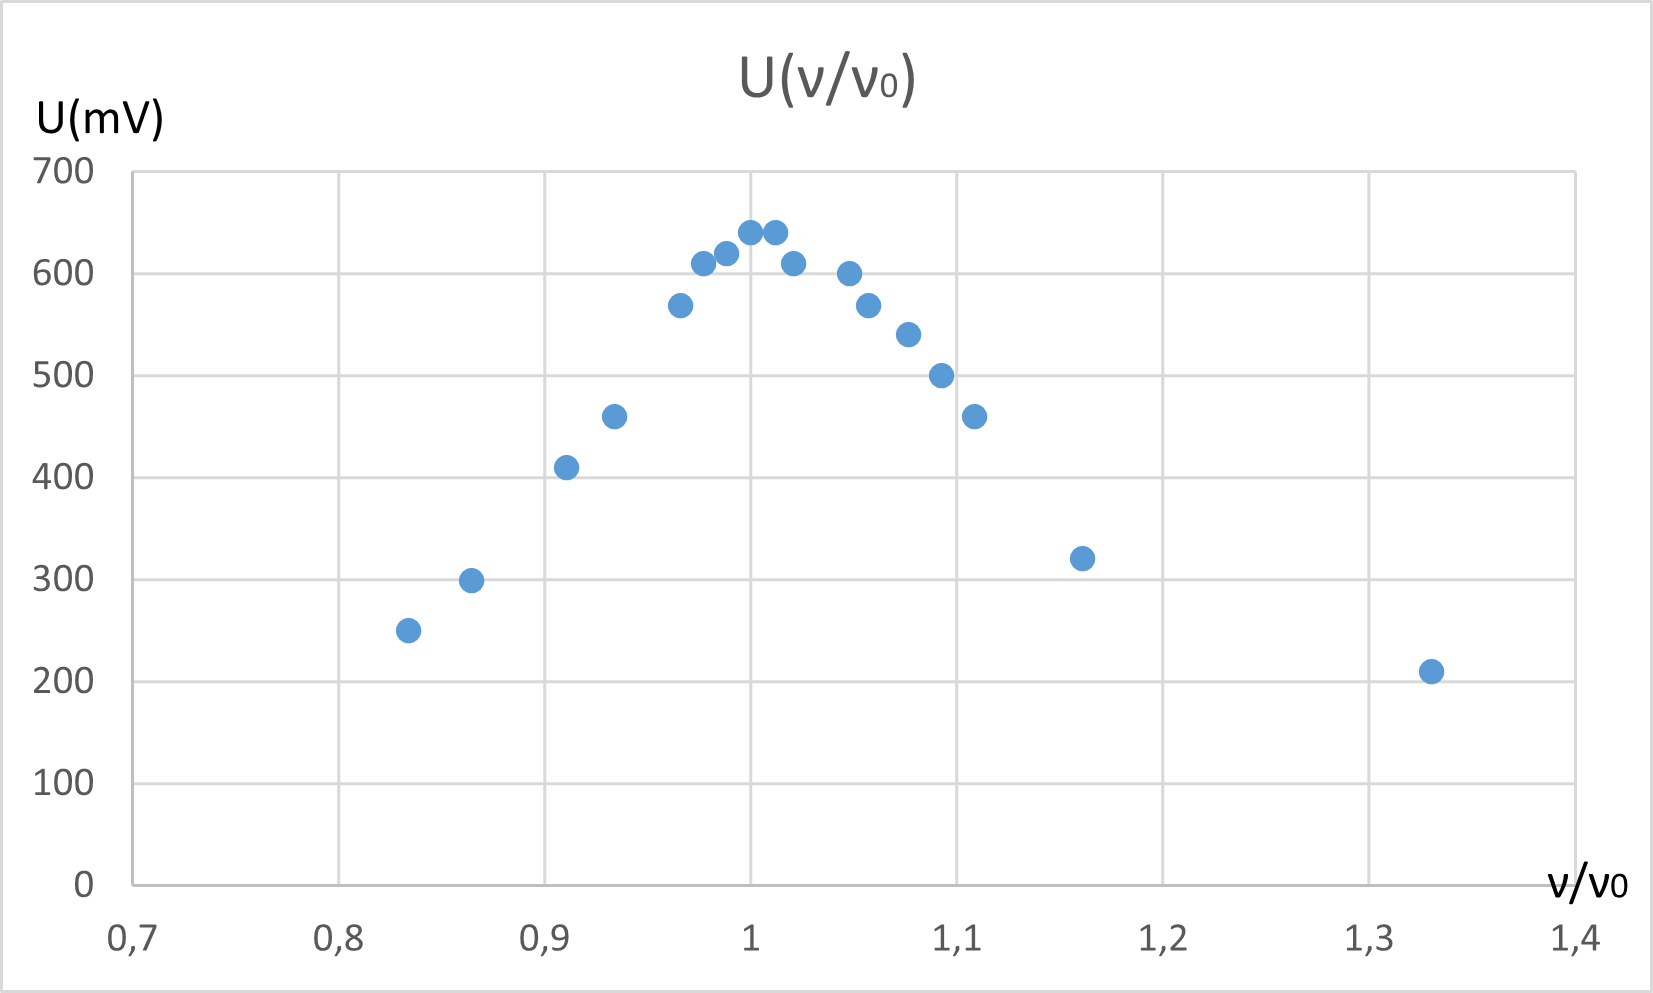
\includegraphics[width=\textwidth]{R = 20.png}
    \caption{R = 20 $\Omega$}
    \label{fig:galaxy}
\end{figure}

\begin{figure}[htp]
    \centering
    \includegraphics[width=\textwidth]{vse.png}
    \caption{Vsi nizi}
    \label{fig:galaxy}
\end{figure}

\begin{figure}[htp]
    \centering
    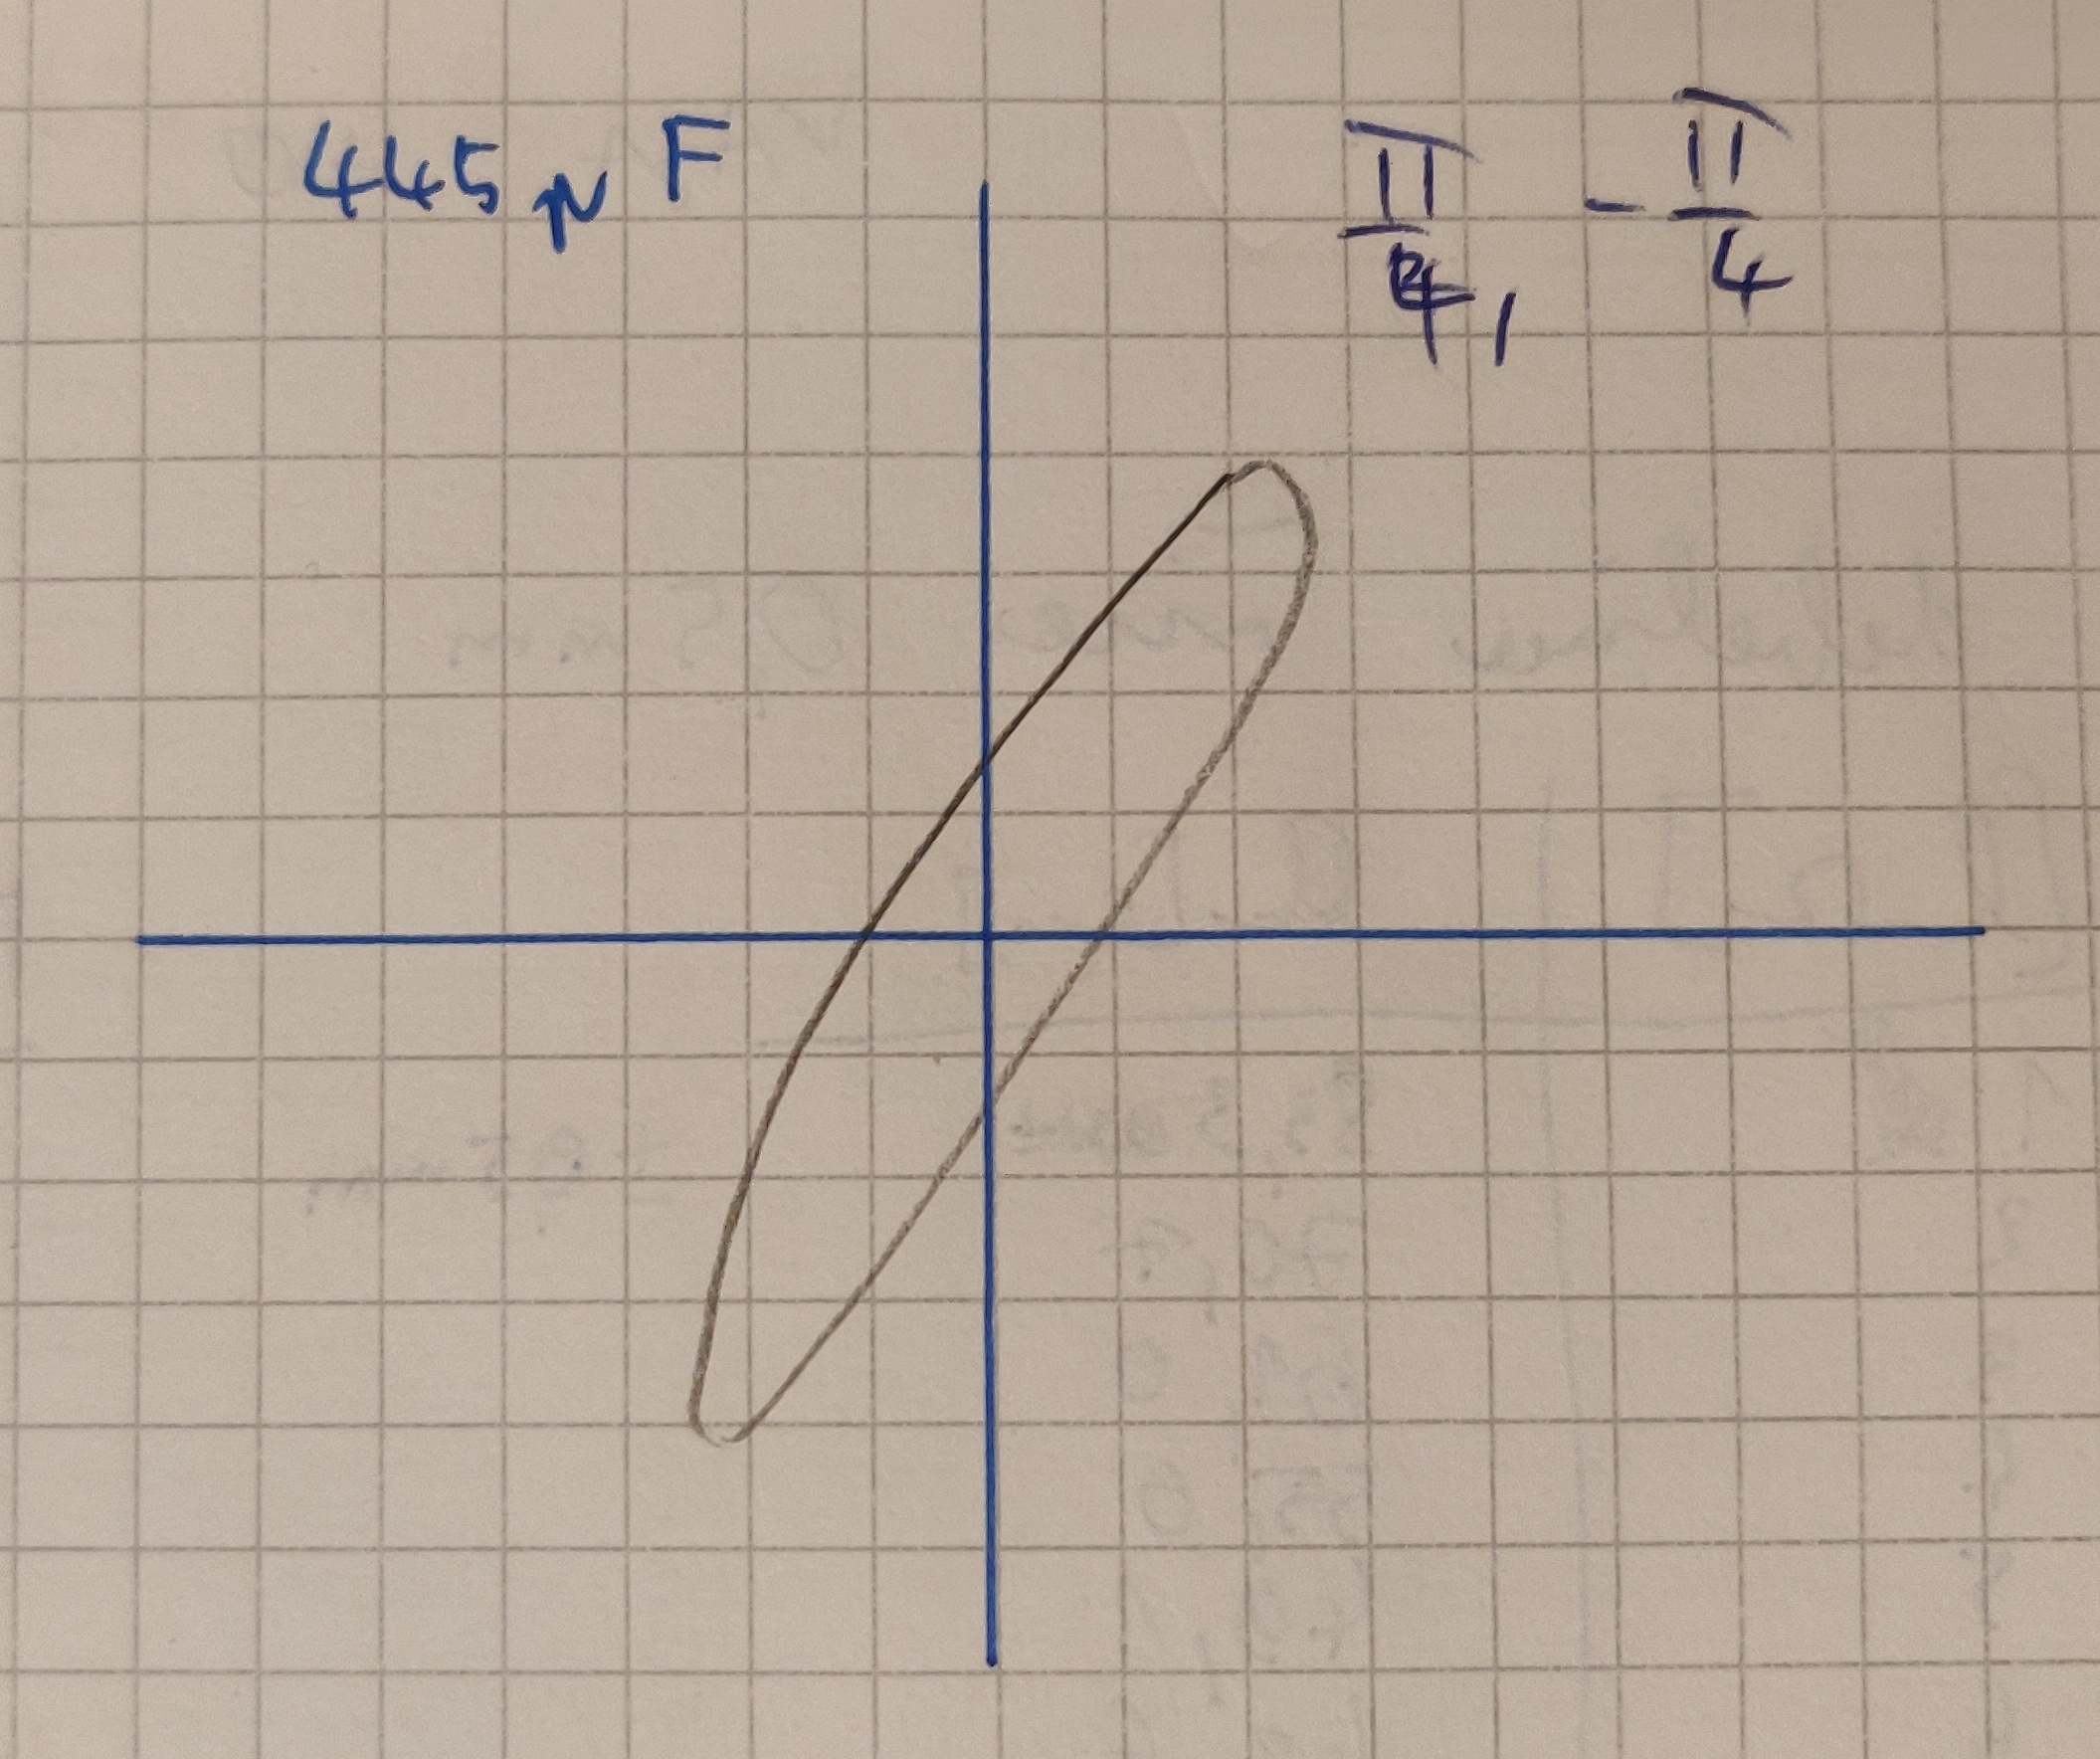
\includegraphics[width=\textwidth]{Lisajeva elipsa1.png}
    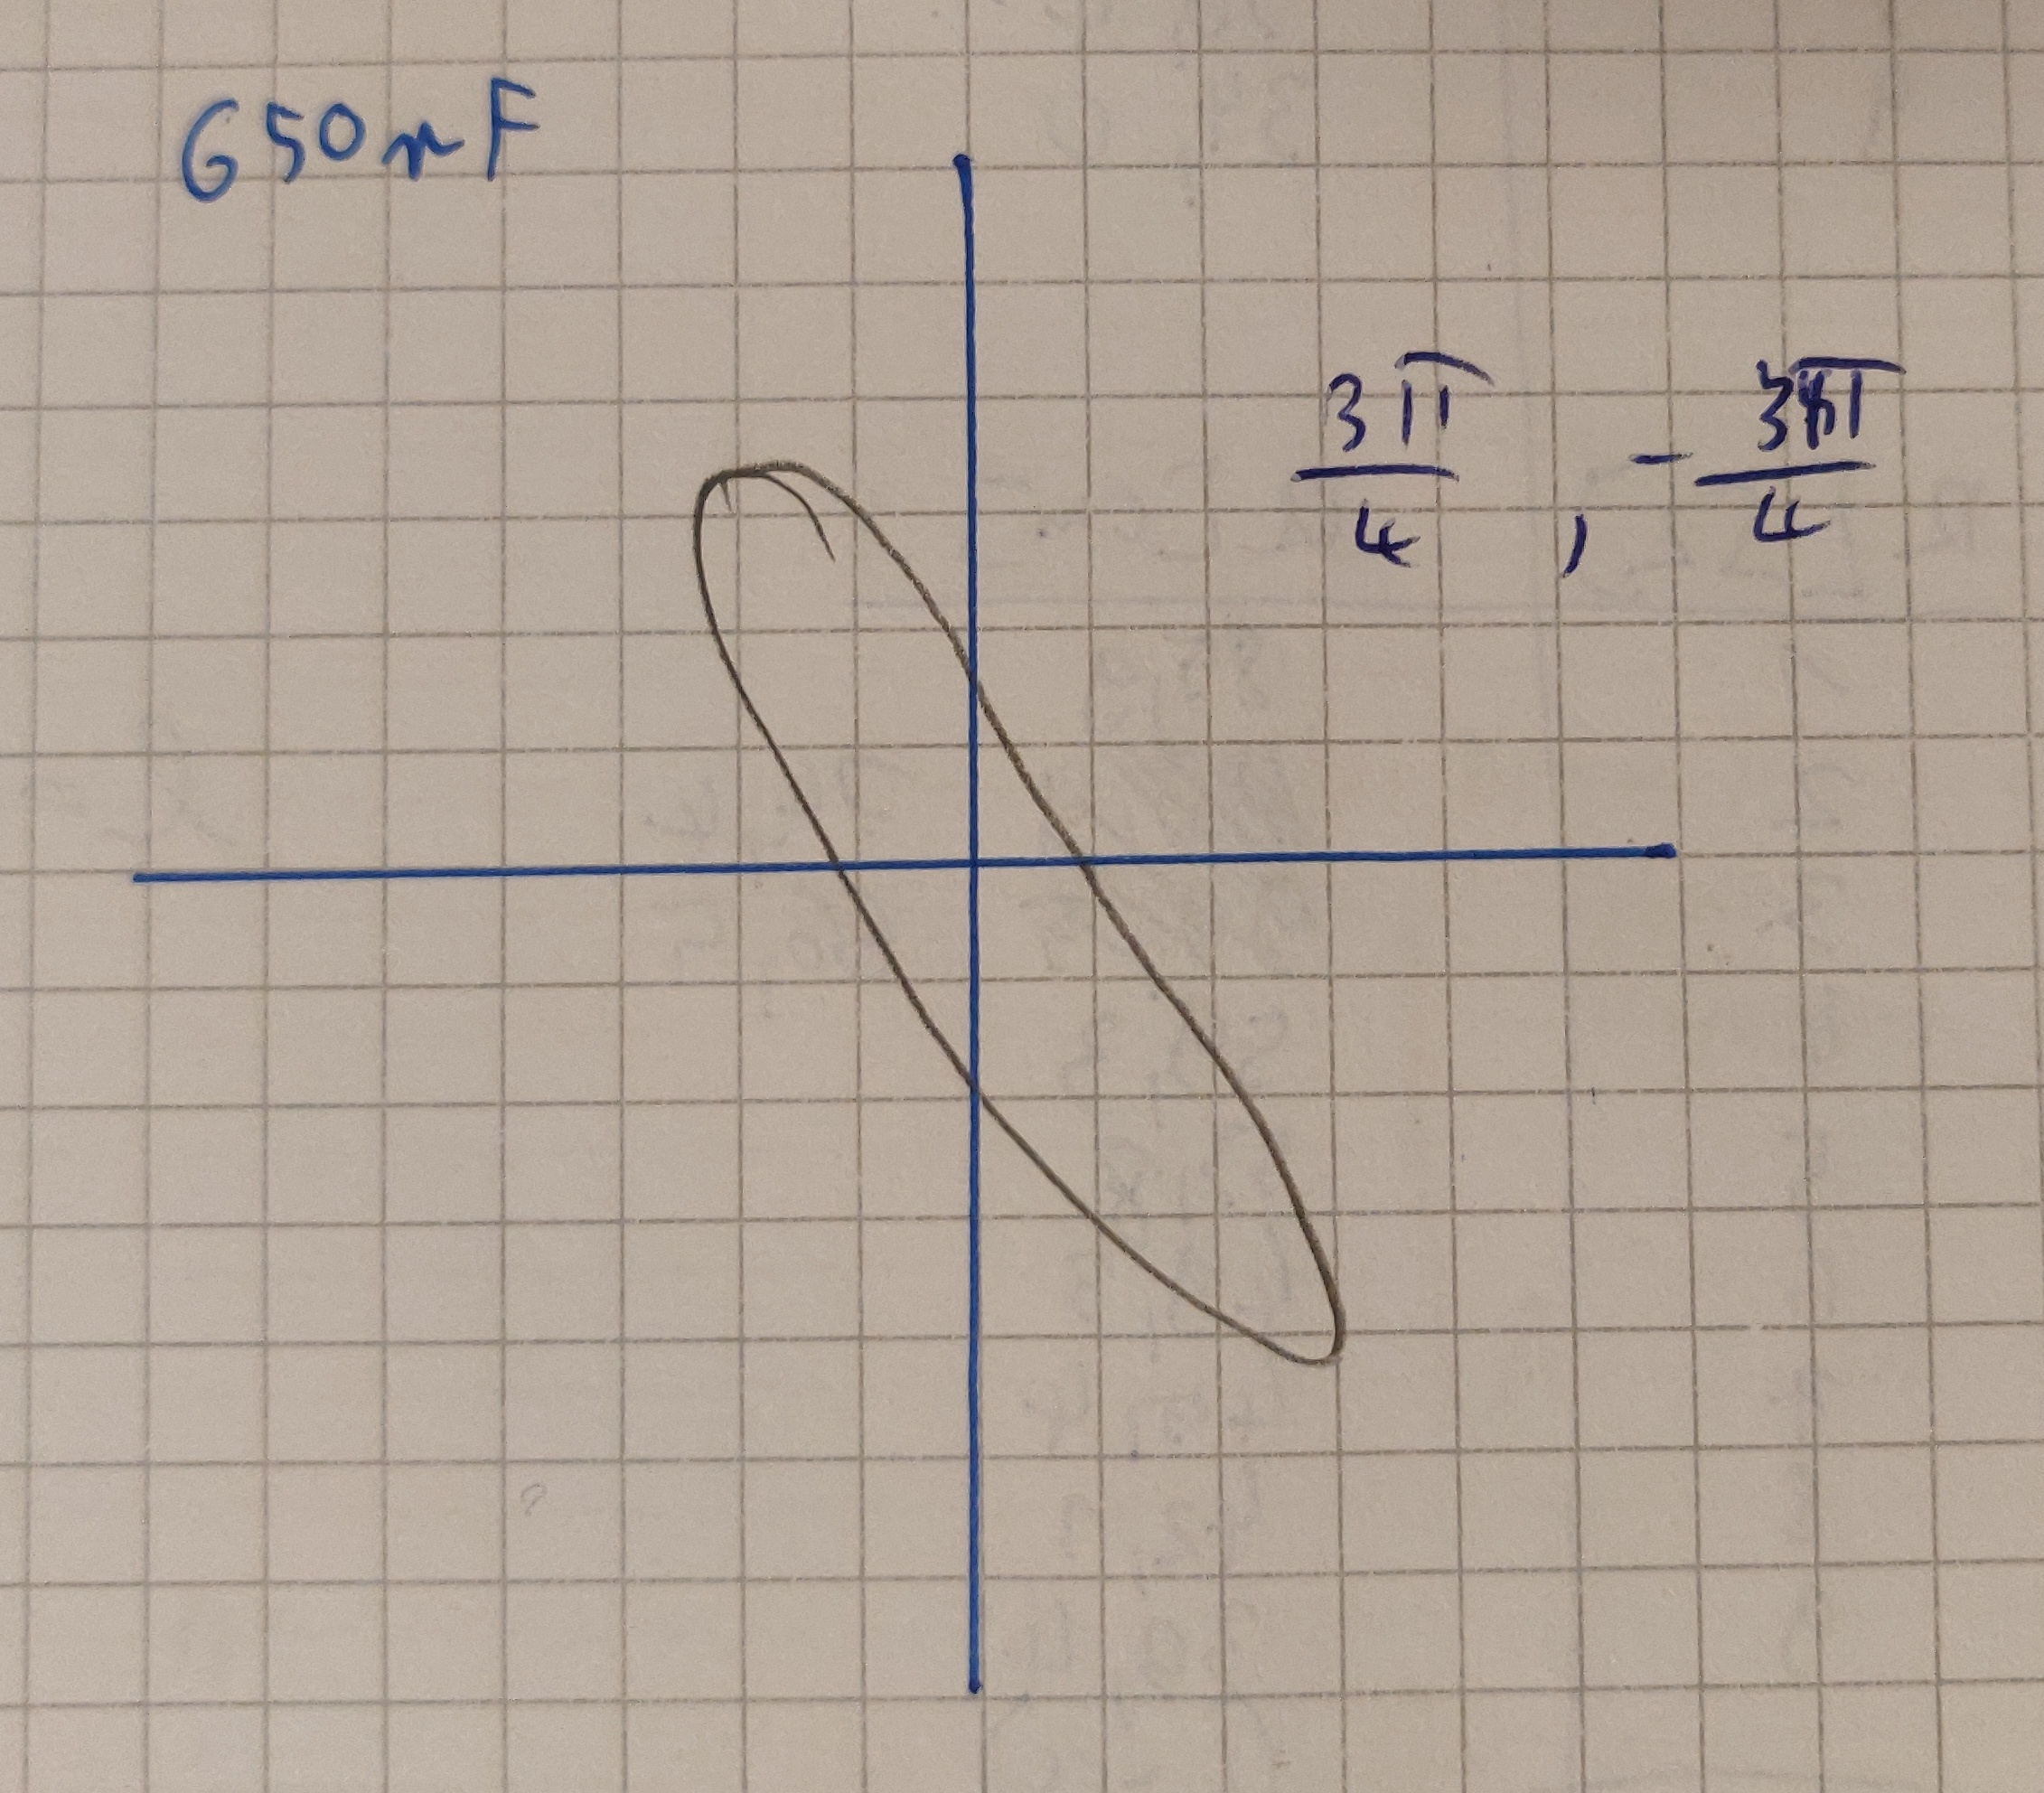
\includegraphics[width=\textwidth]{Lisajeva elipsa2.png}
    \caption{Ko je elipsa, je zamik $\frac{\pi}{4}$, $-\frac{\pi}{4}$, $\frac{3\pi}{4}$ ali $-\frac{3\pi}{4}$}
    \label{fig:galaxy}
\end{figure}

\begin{figure}[htp]
    \centering
    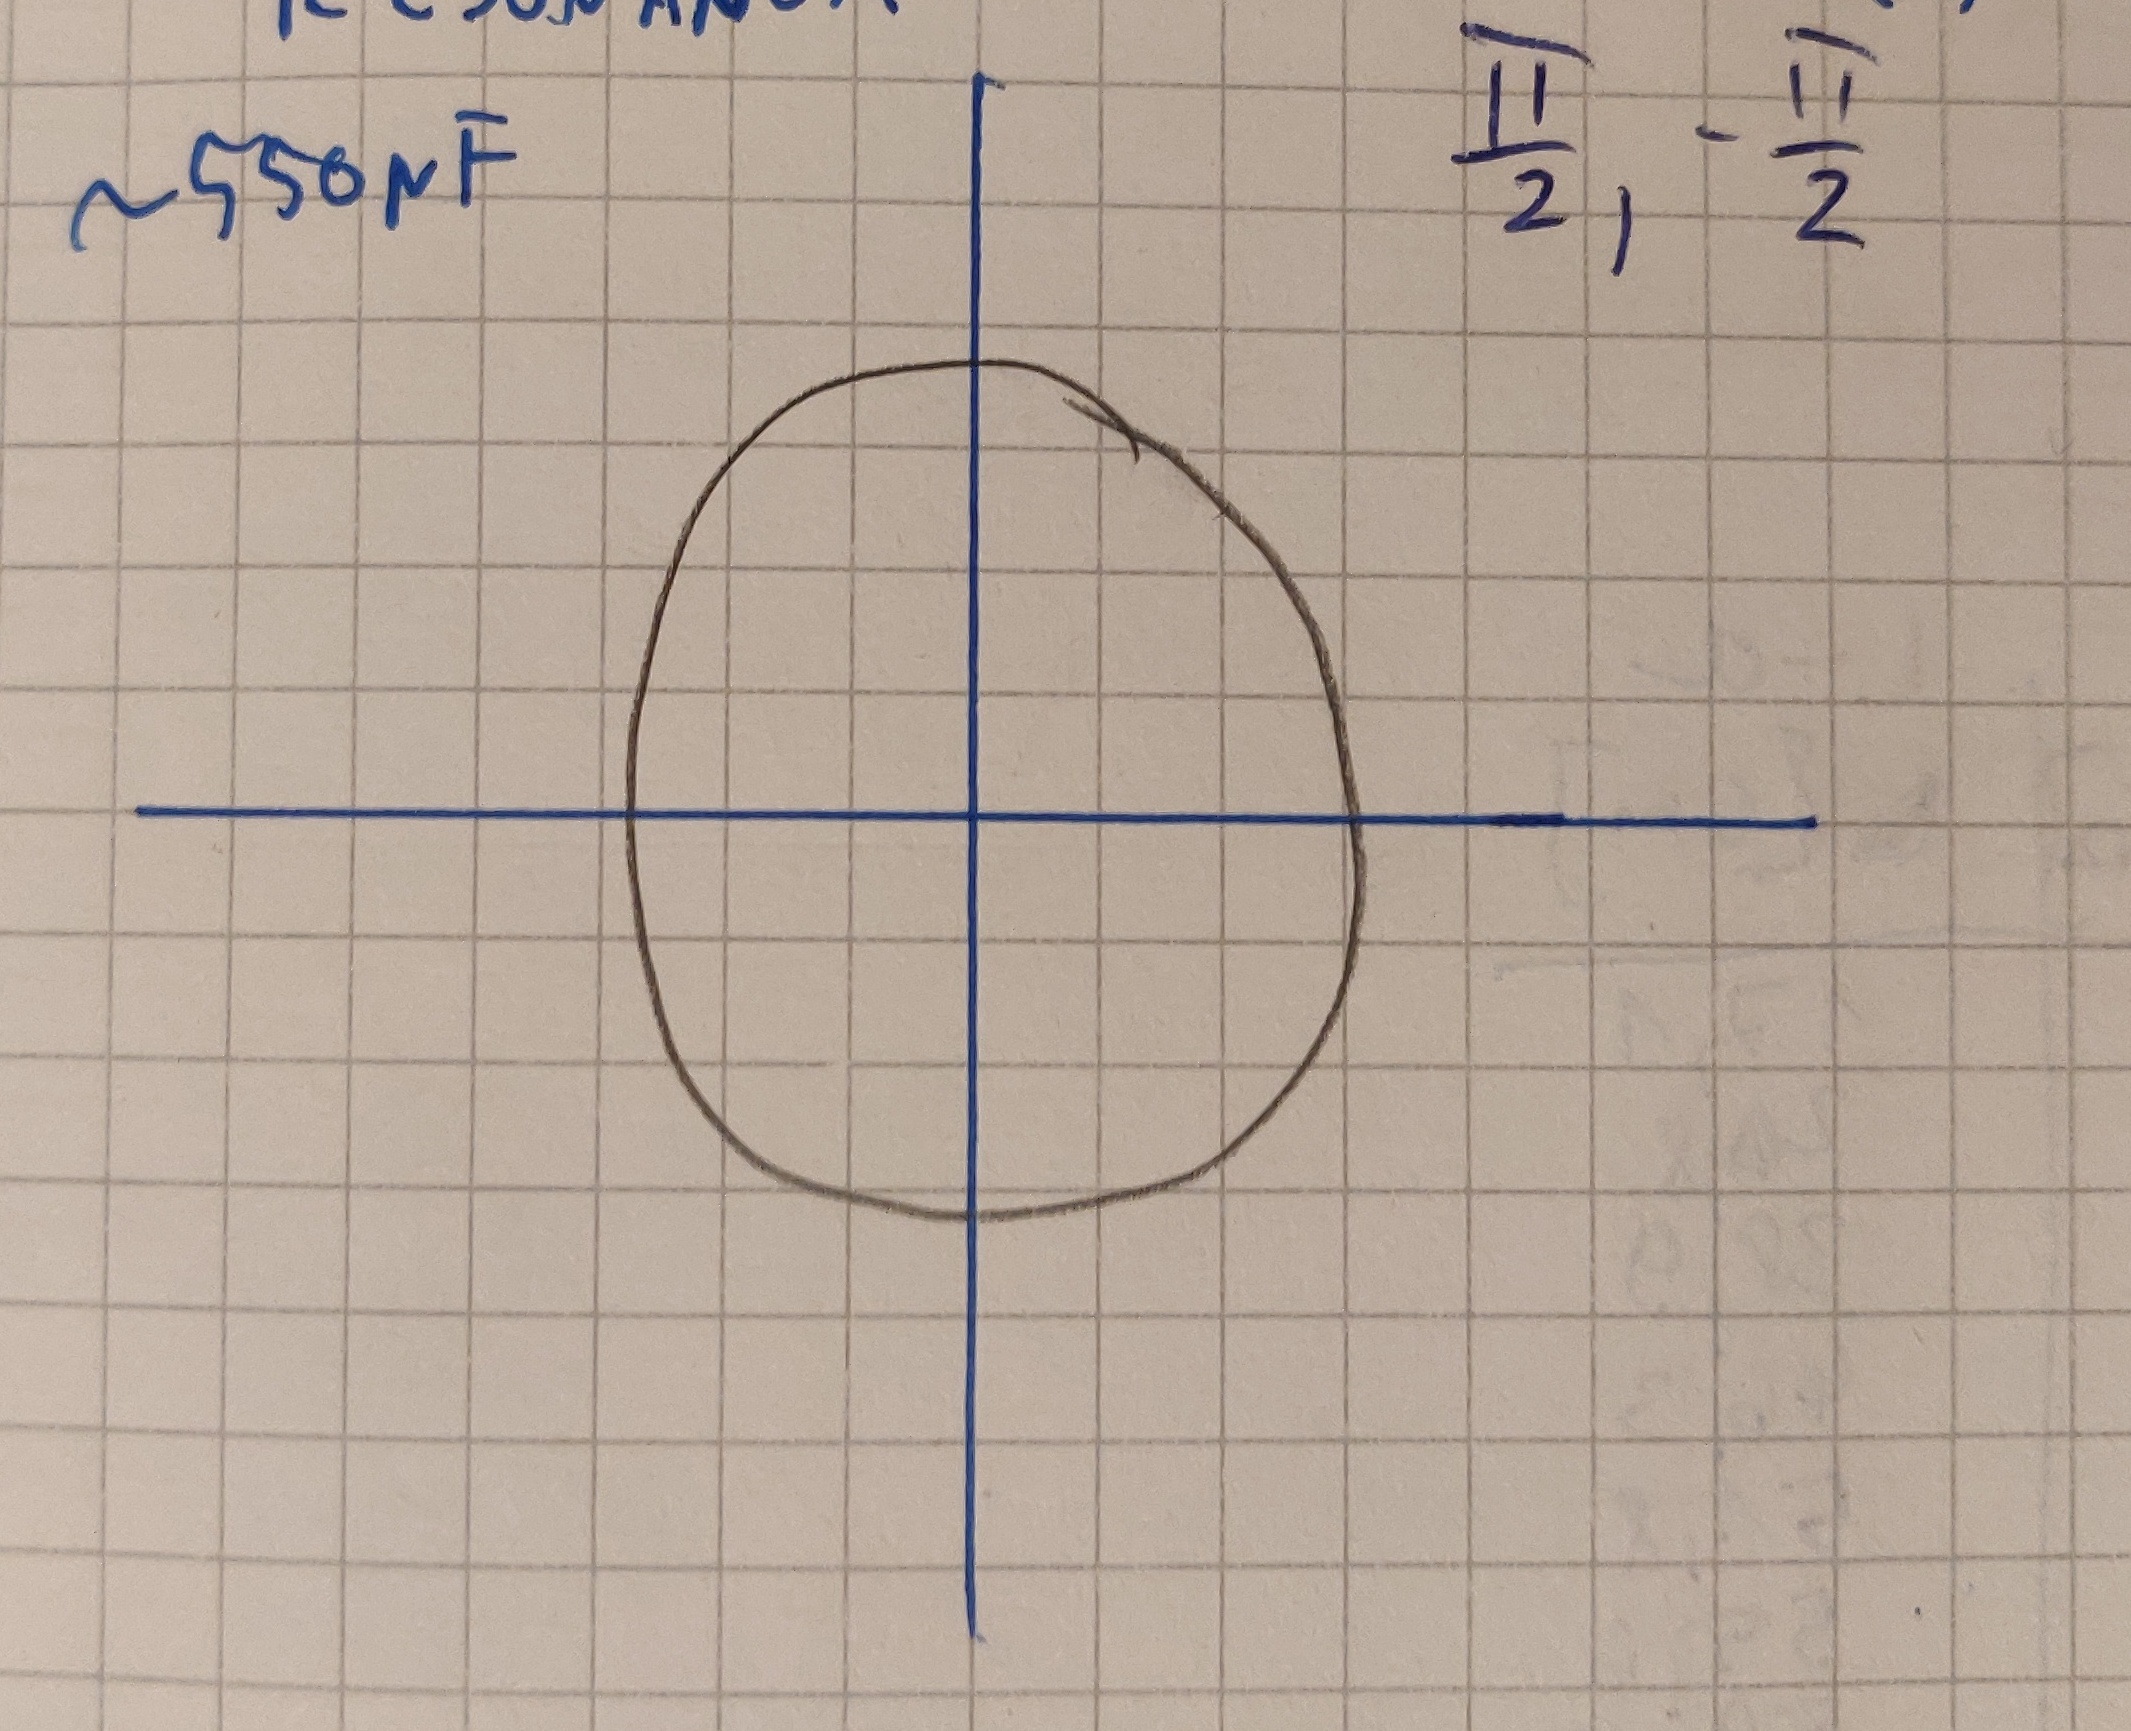
\includegraphics[width=\textwidth]{Lisajeva krog.png}
    \caption{Ko je krog, je resonančno valovanje in je fazni odmik enak $\frac{\pi}{2}$ ali $-\frac{\pi}{2}$}
    \label{fig:galaxy}
\end{figure}

\begin{figure}[htp]
    \centering
    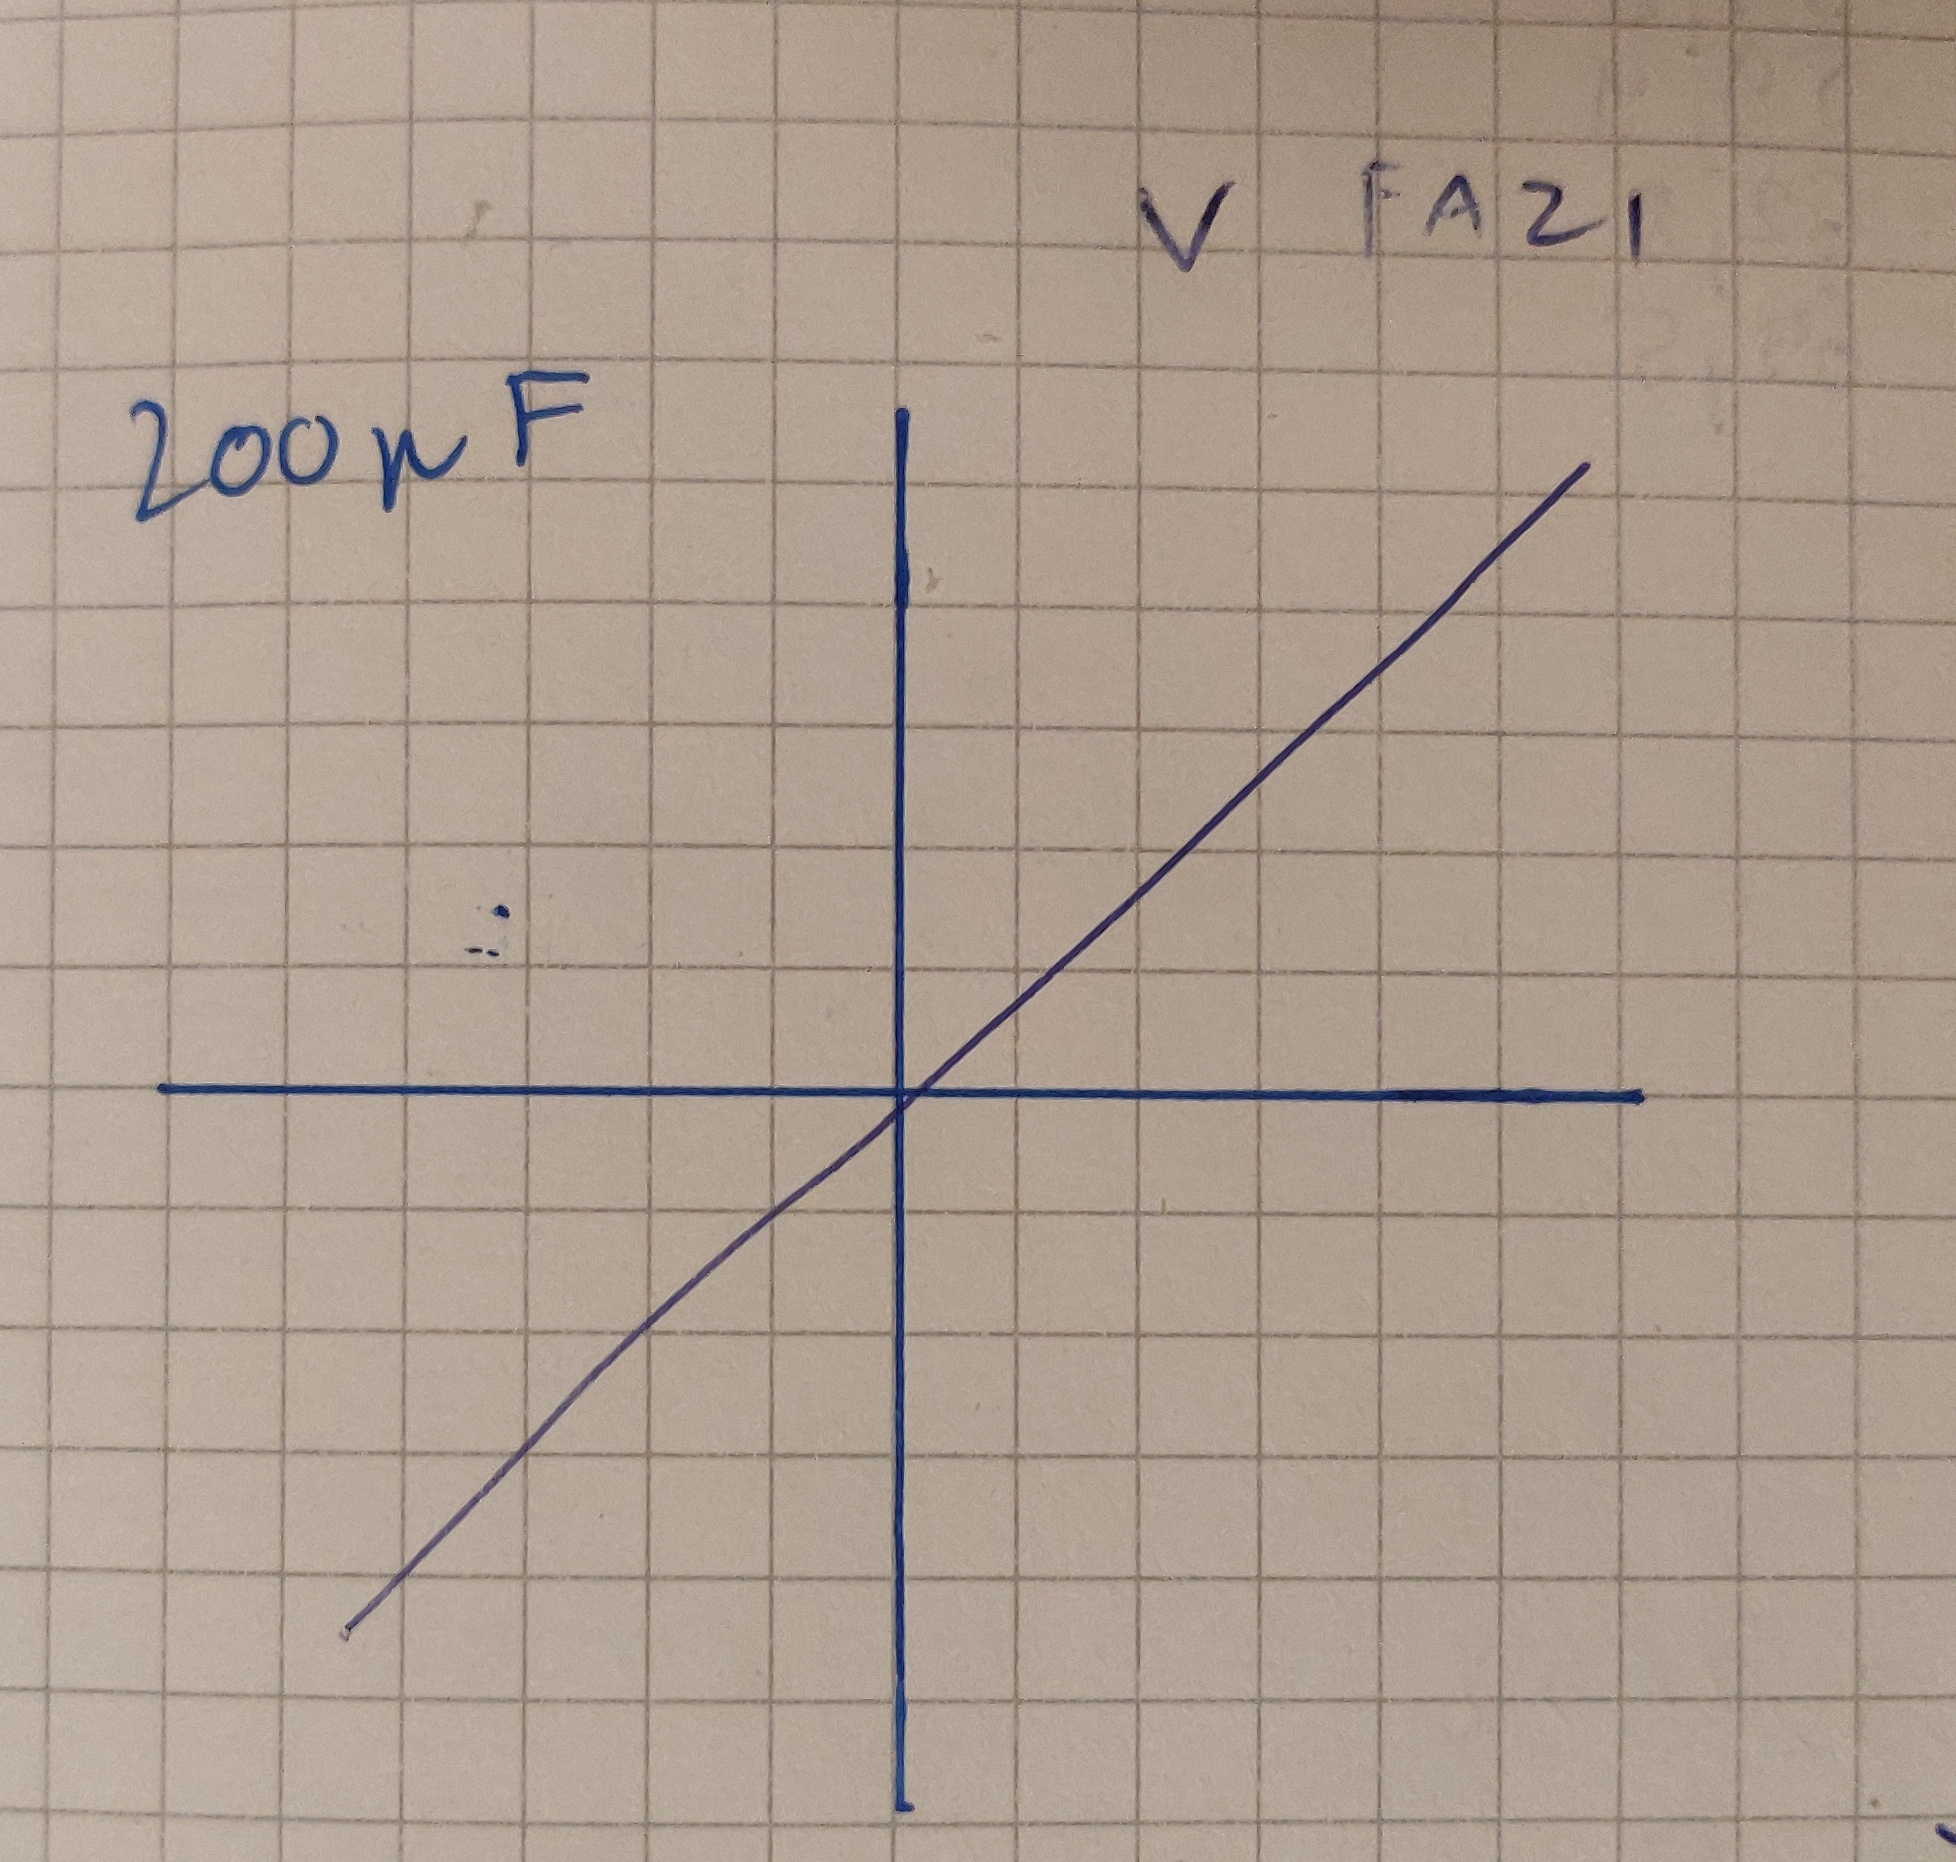
\includegraphics[width=\textwidth]{Lisajeva skor premica1.png}
    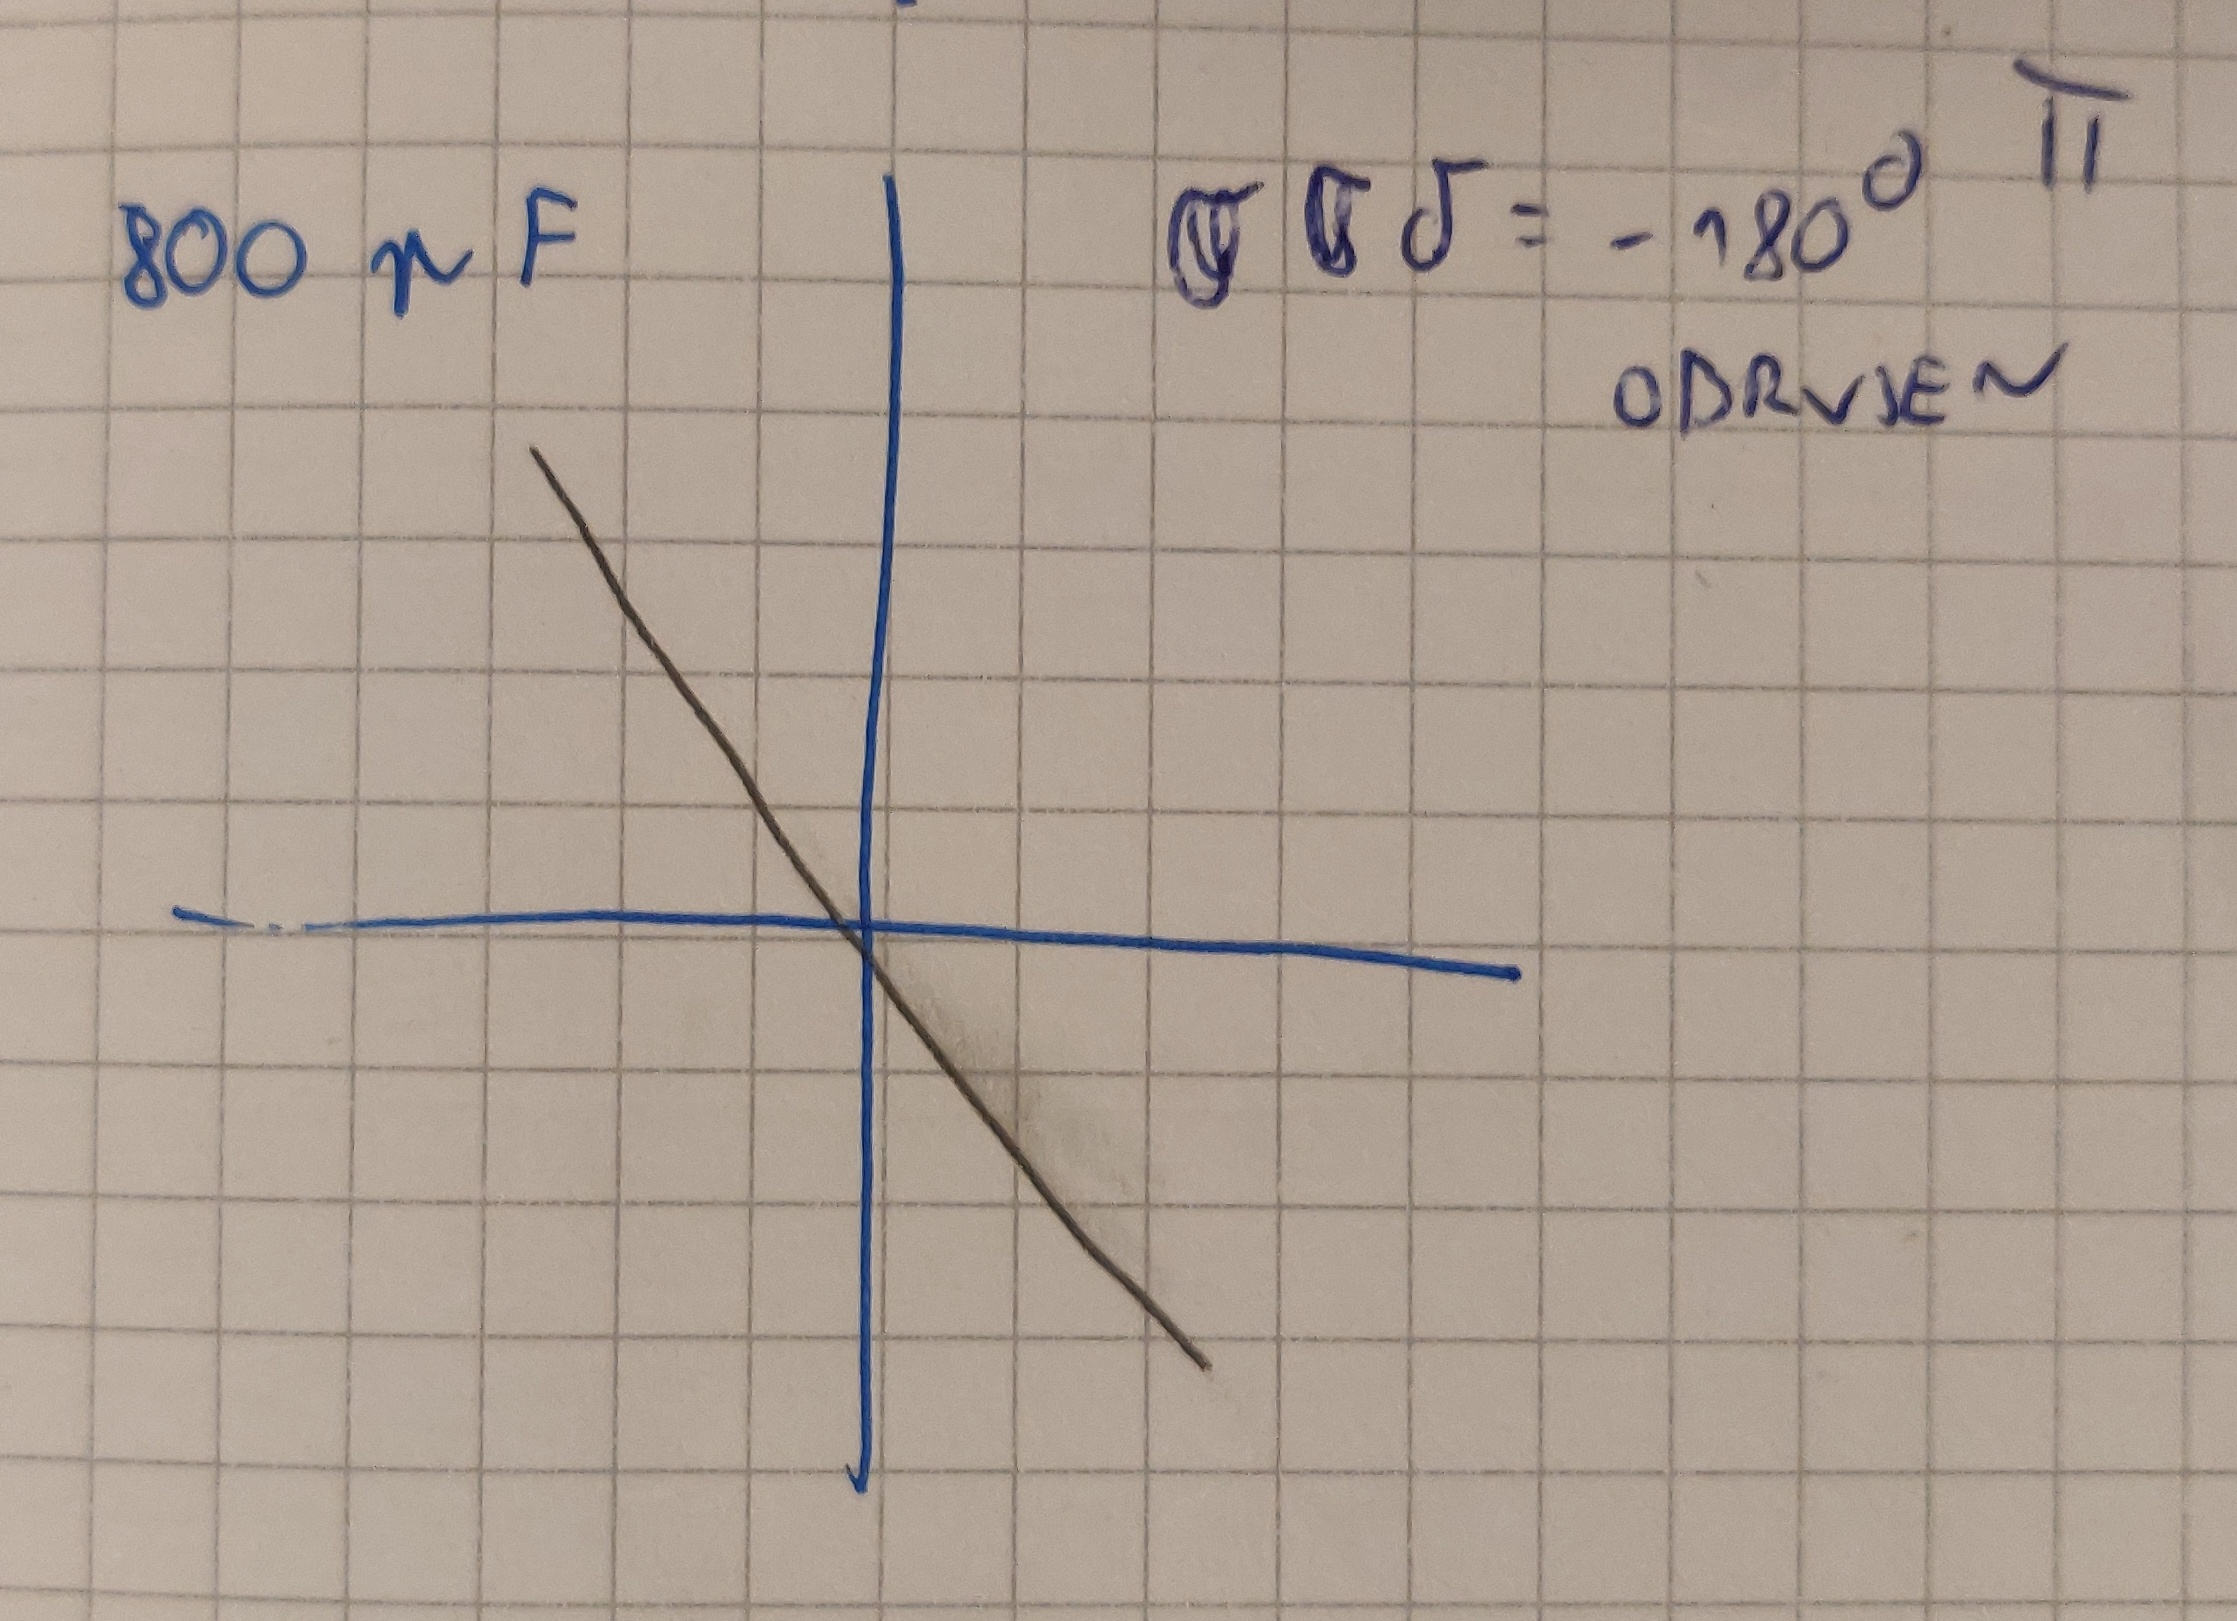
\includegraphics[width=\textwidth]{Lisajeva skor premica2.png}
    \caption{Ko je premica, je fazni odmik enak 0 ali $\pi$}
    \label{fig:galaxy}
\end{figure}

\end{document}